% =============================================================================
%  Rapport — Mini-cloud Zero Trust et banque de démonstration « ZT Bank »
%  Compilation : xelatex rapport.tex (deux fois)  ou  pdflatex rapport.tex (deux fois)
%  (Overleaf : n'importe quel compilateur). Les captures sont lues dans ../screens/.
% =============================================================================
\documentclass[11pt,a4paper]{article}

\usepackage{iftex}
\ifXeTeX
  \usepackage{fontspec}
  \usepackage{polyglossia}
  \setdefaultlanguage{french}
\else\ifLuaTeX
  \usepackage{fontspec}
  \usepackage{polyglossia}
  \setdefaultlanguage{french}
\else
  \usepackage[utf8]{inputenc}
  \usepackage[T1]{fontenc}
  \usepackage{lmodern}
  \usepackage[french]{babel}
\fi\fi

\usepackage[margin=2.3cm]{geometry}
\usepackage{microtype}
\usepackage{xcolor}
\usepackage{graphicx}
\usepackage{booktabs}
\usepackage{tabularx}
\usepackage{longtable}
\usepackage{array}
\usepackage{enumitem}
\usepackage{float}
\usepackage{caption}
\usepackage{fancyhdr}
\usepackage{listings}
\usepackage{tikz}
\usetikzlibrary{arrows.meta,positioning,fit,backgrounds,calc,shapes.geometric}
\usepackage[hidelinks]{hyperref}

% ---------------------------------------------------------------- à compléter --
\newcommand{\titre}{Mini-cloud \emph{Zero Trust}\\[2pt]et banque de démonstration « ZT Bank »}
\newcommand{\auteurs}{\textit{Prénom Nom} \quad\&\quad \textit{Prénom Nom}}   % à compléter
\newcommand{\cours}{\textit{Intitulé du cours — Établissement}}               % à compléter
\newcommand{\depot}{\url{https://github.com/Yassminefeki/PQC-Cloud-Lab}}
% -----------------------------------------------------------------------------

\definecolor{zt}{HTML}{0F3D3E}
\definecolor{ztlight}{HTML}{E8F1EF}
\definecolor{ok}{HTML}{1B7A4B}
\definecolor{bad}{HTML}{B3261E}
\definecolor{code}{HTML}{F5F5F2}

\lstset{basicstyle=\ttfamily\small, backgroundcolor=\color{code}, frame=single, rulecolor=\color{black!15},
        columns=fullflexible, keepspaces=true, breaklines=true, showstringspaces=false,
        xleftmargin=4pt, xrightmargin=4pt, aboveskip=6pt, belowskip=6pt,
        literate={é}{{\'e}}1 {è}{{\`e}}1 {à}{{\`a}}1 {ê}{{\^e}}1 {ç}{{\c{c}}}1 {É}{{\'E}}1 {ô}{{\^o}}1 {—}{{---}}1 {→}{{$\rightarrow$}}1 {×}{{$\times$}}1}

\pagestyle{fancy}
\fancyhf{}
\fancyhead[L]{\small\color{black!60}ZT Bank — mini-cloud Zero Trust}
\fancyhead[R]{\small\color{black!60}\leftmark}
\fancyfoot[C]{\small\thepage}
\renewcommand{\headrulewidth}{0.3pt}

\setlist{itemsep=2pt, topsep=4pt}
\newcolumntype{L}{>{\raggedright\arraybackslash}X}
\newcommand{\cmd}[1]{\texttt{#1}}
\newcommand{\defended}{\textcolor{ok}{\textbf{DEFENDED}}}
% Captures de la démo (docs/screens/demo/) : incluses si présentes. Pour voir celles qui manquent,
% décommenter la ligne suivante.
% \def\montrermanquantes{}
\newcommand{\capture}[3][0.95]{%
  \IfFileExists{../screens/demo/#2}{%
    \begin{figure}[H]\centering\includegraphics[width=#1\linewidth]{../screens/demo/#2}\caption{#3}\end{figure}}{%
    \ifdefined\montrermanquantes
      \begin{center}\fcolorbox{black!30}{black!3}{\parbox{0.9\linewidth}{\centering\small\color{black!60}%
        Capture à ajouter : \texttt{docs/screens/demo/\detokenize{#2}}\\ #3}}\end{center}\fi}}

\begin{document}
\sloppy

% ================================================================= titre ==
\begin{titlepage}
  \centering
  \vspace*{2.5cm}
  {\color{zt}\rule{\linewidth}{1.2pt}}\\[14pt]
  {\Huge\bfseries\color{zt}\titre\par}
  \vspace{10pt}
  {\color{zt}\rule{\linewidth}{1.2pt}}\\[24pt]
  {\Large Rapport de projet\par}
  \vspace{2.2cm}
  {\large \auteurs\par}
  \vspace{8pt}
  {\cours\par}
  \vspace{2.2cm}
  \begin{minipage}{0.82\linewidth}
  \small
  \textbf{Résumé.} Nous avons construit, sur un seul ordinateur portable, un petit cloud de six
  machines virtuelles qui applique le modèle \emph{zero trust} : aucune machine n'est crue sur sa
  seule position réseau, chaque requête est authentifiée par un certificat à chaque saut, et tout
  ce qui n'est pas explicitement permis est refusé et journalisé. Les règles sont écrites une seule
  fois dans un fichier de politique, puis générées en configuration (pare-feu, mTLS, PKI, base de
  données) et vérifiées par plus de 450 tests. Le cloud héberge une banque de démonstration utilisée
  depuis un second ordinateur à travers WireGuard. Onze attaques jouées depuis le cloud et six depuis le
  poste distant sont toutes repoussées ; la révocation d'un certificat volé prend effet en moins d'une
  minute, sans redémarrage.
  \end{minipage}
  \vfill
  {\small Code source : \depot\par}
  \vspace{3pt}
  {\small Vidéo de démonstration : \texttt{docs/video/zt-bank-demo.mp4} (3~min~50)\par}
  \vspace{6pt}
  {\small \today\par}
\end{titlepage}

\tableofcontents
\newpage

% ============================================================ 1. analyse ==
\section{Analyse du sujet}

\subsection{Le besoin}
Le modèle classique « château fort » fait confiance à tout ce qui est à l'intérieur du périmètre :
une fois franchi le pare-feu, un attaquant circule librement. Le modèle \emph{zero trust}
(NIST SP~800-207) supprime cette confiance implicite : chaque accès doit être authentifié,
autorisé selon le moindre privilège et journalisé, quelle que soit sa provenance.

Le sujet demande de mettre ce modèle en œuvre de bout en bout sur du matériel personnel : un
ordinateur joue le rôle du \emph{cloud} (hyperviseur de six machines virtuelles), un second celui
du poste de travail des utilisateurs. Il faut que l'ensemble soit \textbf{reproductible},
\textbf{vérifiable} et qu'aucun secret ne se retrouve dans le dépôt de code.

\subsection{Contraintes retenues}
\begin{center}
\begin{tabularx}{\linewidth}{@{}p{5.2cm}L@{}}
\toprule
\textbf{Contrainte} & \textbf{Conséquence dans le projet}\\
\midrule
Un seul ordinateur pour le cloud & KVM/libvirt, réseaux virtuels isolés, 7~Go de RAM pour les VM\\
Un second poste pour l'utilisateur & tunnel WireGuard ; ce poste n'est pas administré par le dépôt\\
Reproductible & tout est du code : Terraform, Ansible, générateur Python, \cmd{make}\\
Vérifiable & chaque étape a ses tests hors ligne et en direct\\
Aucun secret dans Git & clés et mots de passe générés par Ansible dans un dossier ignoré par Git\\
Indépendant du Wi-Fi & aucune adresse Wi-Fi écrite : nom mDNS côté client, filtrage par \emph{nom d'interface} côté hôte\\
Démarche incrémentale & 14 étapes (0 à 13), chacune avec \cmd{make <étape>} et \cmd{make test-<N>}\\
\bottomrule
\end{tabularx}
\end{center}

\subsection{Des principes aux mécanismes}
\begin{center}
\begin{tabularx}{\linewidth}{@{}p{4.6cm}L@{}}
\toprule
\textbf{Principe zero trust} & \textbf{Mécanisme mis en place}\\
\midrule
Ne jamais faire confiance au réseau & pare-feu \emph{default drop} sur \textbf{chaque} VM ; aucune VM n'est routée vers une autre\\
Authentifier chaque requête & mTLS en TLS~1.3 à chaque saut, base de données comprise\\
Identités fortes et courtes & certificats SPIFFE de 24~h (1~h pour le robot) émis par une CA interne\\
Moindre privilège & listes d'autorisation par service, routes par rôle, rôle SQL sans écriture, RLS\\
Supposer la compromission & chaque couche revérifie ; révocation en moins d'une minute ; \emph{fail-closed}\\
Tout journaliser & refus journalisés avec l'identité réelle à chaque couche ; audit en base ; \cmd{make audit}\\
\bottomrule
\end{tabularx}
\end{center}

\subsection{Le cas d'usage : ZT Bank}
Pour que la sécurité porte sur quelque chose de concret, le cloud héberge une petite banque.
Ses utilisateurs n'ont \textbf{pas de mot de passe} : leur certificat client est leur identité.
\begin{itemize}
  \item \textbf{Alice} et \textbf{Bob}, clients : consultent leurs comptes, font des virements ;
  \item \textbf{Dev}, support : voit la santé du système, jamais les données des clients ;
  \item \textbf{statements}, un robot : produit les relevés, certificat d'une heure lié à sa machine ;
  \item \textbf{PayFlow}, partenaire de paiement : notifie des paiements depuis Internet, sans VPN.
\end{itemize}

\subsection{Hors périmètre}
Haute disponibilité, sécurité propre du poste client et du navigateur, cryptographie
post-quantique (voir les perspectives), services du portable hôte étrangers à la banque.

% =========================================================== 2. conception ==
\section{Conception}

\subsection{Architecture}

\begin{figure}[H]
\centering
\begin{tikzpicture}[
  node distance=6mm and 8mm,
  vm/.style={draw=zt, fill=ztlight, rounded corners=2pt, minimum width=3.3cm, minimum height=9mm, align=center, font=\small},
  ext/.style={draw=black!50, fill=white, rounded corners=2pt, minimum width=3.0cm, minimum height=9mm, align=center, font=\small},
  net/.style={font=\scriptsize\itshape, text=black!60},
  flow/.style={-{Latex[length=2mm]}, thick, zt},
  mgmt/.style={-{Latex[length=2mm]}, dashed, black!45}]
  \node[ext] (rc) {Poste distant\\\scriptsize Firefox, WireGuard};
  \node[ext, right=2.2cm of rc] (host) {Cloud host\\\scriptsize DNAT par nom d'interface};
  \node[ext, below=of rc] (pf) {PayFlow\\\scriptsize Internet, sans VPN};
  \node[vm, below=1.2cm of host] (gw) {VM1 \textbf{gateway}\\\scriptsize wg0 10.10.0.1};
  \node[vm, below=of gw] (fe) {VM2 \textbf{frontend}\\\scriptsize :8443 site · :8444 partenaire};
  \node[vm, below=of fe] (sa) {VM3 \textbf{service-a}\\\scriptsize core :9443};
  \node[vm, below=of sa] (sb) {VM4 \textbf{service-b}\\\scriptsize ledger :9443};
  \node[vm, below=of sb] (db) {VM5 \textbf{database}\\\scriptsize PostgreSQL :5432};
  \node[vm, right=1.6cm of sa] (ca) {VM6 \textbf{ca}\\\scriptsize step-ca :9000};
  \draw[flow] (rc) -- node[above, font=\scriptsize]{UDP 51820} (host);
  \draw[flow] (pf.east) -| node[pos=0.25, below, font=\scriptsize]{TCP 8444} ($(host.south)+(-0.6,0)$);
  \draw[flow] (host) -- (gw);
  \draw[flow] (gw) -- node[right, font=\scriptsize]{tunnel → :8443 seulement} (fe);
  \draw[flow] (fe) -- node[right, font=\scriptsize]{mTLS} (sa);
  \draw[flow] (sa) -- node[right, font=\scriptsize]{mTLS} (sb);
  \draw[flow] (sb) -- node[right, font=\scriptsize]{TLS 1.3 + certificat} (db);
  \draw[mgmt] (fe.east) -| (ca.north);
  \draw[mgmt] (sa) -- (ca);
  \draw[mgmt] (sb.east) -| (ca.south);
  \node[net, left=3mm of fe] {dmz 10.20.0.0/24};
  \node[net, left=3mm of sa] {app 10.30.0.0/24};
  \node[net, left=3mm of db] {data 10.40.0.0/24};
  \node[net, below=1mm of ca] {mgmt 10.50.0.0/24 (pointillés)};
\end{tikzpicture}
\caption{Architecture : six VM sur quatre réseaux isolés ; les flèches pleines sont les seuls flux métier autorisés.}
\end{figure}

Les adresses sont celles des réseaux \emph{virtuels} internes, déclarés dans la politique ; elles
ne dépendent pas du réseau Wi-Fi. Les réseaux dmz, app et data sont isolés et l'hôte n'y a même
pas d'adresse ; seul le gateway route, et seulement du tunnel vers le site.

\subsection{Trois verrous indépendants}
Une requête doit franchir, à chaque saut :
\begin{enumerate}
  \item le \textbf{réseau} : nftables \emph{default drop} en entrée, sortie et transit sur chaque VM ;
        un flux n'est ouvert que si les deux extrémités l'autorisent ; les refus sont silencieux et journalisés ;
  \item le \textbf{transport} : WireGuard (avec clé pré-partagée) depuis l'extérieur, TLS~1.3 uniquement à l'intérieur ;
  \item l'\textbf{identité} : certificat SPIFFE valide, non révoqué, présent dans la liste
        d'autorisation du service, puis route ouverte au rôle de l'appelant.
\end{enumerate}

\subsection{La politique, source unique de vérité}
Toutes les règles sont écrites une seule fois dans \cmd{policy.yaml} : réseaux, nœuds, services,
flux autorisés, PKI, pairs WireGuard, acteurs, rôles, routes, paramètres de la banque. Ce qui
dépend de la machine (nom mDNS, interface réseau, utilisateur SSH) est isolé dans \cmd{env.yaml},
non versionné. Un générateur Python, \cmd{tools/gen\_rules.py}, transforme ces deux fichiers en
toutes les configurations ; Terraform, Ansible et les tests ne lisent que ce résultat.

\begin{figure}[H]
\centering
\begin{tikzpicture}[box/.style={draw=zt, fill=ztlight, rounded corners=2pt, align=center, font=\small, minimum height=8mm},
                    outbox/.style={draw=black!40, rounded corners=1pt, align=left, font=\scriptsize, minimum width=4.6cm},
                    arr/.style={-{Latex[length=2mm]}, thick, zt}]
  \node[box] (p) {policy.yaml};
  \node[box, below=4mm of p] (e) {env.yaml\\\scriptsize(non versionné)};
  \node[box, right=1.4cm of $(p)!0.5!(e)$, minimum width=2.6cm] (g) {gen\_rules.py\\\scriptsize validation + rendu};
  \node[outbox, right=1.4cm of g, yshift=12mm] (o1) {nftables de chaque VM, DNAT de l'hôte};
  \node[outbox, below=1mm of o1] (o2) {mtls.json : identités, listes, routes, CRL};
  \node[outbox, below=1mm of o2] (o3) {pg\_hba / pg\_ident, schéma bancaire};
  \node[outbox, below=1mm of o3] (o4) {PKI : identités, politique d'émission};
  \node[outbox, below=1mm of o4] (o5) {WireGuard, Terraform, inventaire};
  \node[outbox, below=1mm of o5] (o6) {matrice attendue (pour les tests)};
  \draw[arr] (p) -- (g); \draw[arr] (e) -- (g);
  \foreach \o in {o1,o2,o3,o4,o5,o6} \draw[arr] (g.east) -- (\o.west);
\end{tikzpicture}
\caption{Une politique, toutes les configurations : les tests comparent ensuite le réel au généré.}
\end{figure}

Le générateur \textbf{refuse} une politique incohérente : adresse IP comme point d'entrée, flux
d'administration hors du réseau mgmt, flux métier sur mgmt, adresse hors de son réseau, doublon,
flux entre deux VM sans réseau commun, acteur sans route, durée de certificat au-delà du maximum.

\subsection{Flux et acteurs}
\begin{center}
\begin{tabularx}{\linewidth}{@{}lll L@{}}
\toprule
\textbf{Flux} & \textbf{De} & \textbf{Vers} & \textbf{Rôle}\\
\midrule
wg-ingress & Internet & gateway UDP 51820 & entrée du VPN\\
client-frontend & tunnel & frontend 8443 & site et API des acteurs\\
partner-webhook & Internet & frontend 8444 & notifications PayFlow (DNAT + SNAT)\\
frontend → service-a & frontend & service-a 9443 & règles métier\\
service-a → service-b & service-a & service-b 9443 & grand livre\\
service-b → database & service-b & PostgreSQL 5432 & seul client de la base\\
admin-ssh, pki, packages & hôte / VM & mgmt & administration, enrôlement, paquets\\
\bottomrule
\end{tabularx}
\end{center}

\begin{center}
\begin{tabularx}{\linewidth}{@{}llL l@{}}
\toprule
\textbf{Acteur} & \textbf{Rôle} & \textbf{Droits} & \textbf{Arrive par}\\
\midrule
alice, bob & customer & ses comptes, son historique, ses virements & tunnel\\
dev & staff & santé du système, jamais de données client & tunnel\\
statements & bot & relevés ; certificat 1~h lié à son appareil & tunnel (espace réseau dédié)\\
payflow & partner & \cmd{POST /webhook} signé uniquement & Internet\\
\bottomrule
\end{tabularx}
\end{center}

\subsection{Identités et PKI}
La CA interne (step-ca) émet des certificats SPIFFE (\cmd{spiffe://cloud.local/<nom>}) de 24~h.
La clé d'une VM est générée \emph{sur la VM} et n'en sort jamais ; l'enrôlement utilise un jeton à
usage unique créé sur la CA, si bien que le mot de passe du provisionneur ne quitte jamais la VM
\cmd{ca}. La CA applique elle-même une politique d'émission générée : elle refuse tout nom, toute
adresse ou toute durée que la politique ne prévoit pas. Les certificats sont renouvelés
automatiquement huit heures avant expiration.

\subsection{Le parcours d'un virement}
\begin{enumerate}
  \item Alice, dans Firefox, envoie \cmd{POST /api/transfers} dans le tunnel ;
  \item le gateway ne laisse passer que vers \cmd{frontend:8443} ;
  \item le frontend vérifie le certificat (chaîne, révocation, identité, route, CSRF, débit) et
        déduit « client = alice » \textbf{du certificat seulement} ;
  \item service-a vérifie que l'appelant est le frontend, revérifie le rôle et les plafonds ;
  \item service-b vérifie que l'appelant est service-a et appelle \cmd{bank.transfer()} ;
  \item la fonction SQL contrôle propriété du compte, plafond, limite journalière, solde sous verrou,
        idempotence, écrit en partie double et ajoute une ligne d'audit portant l'identité SPIFFE.
\end{enumerate}
Le grand livre est \emph{append-only} (un déclencheur refuse toute modification, même à
l'administrateur) et la lecture passe par une sécurité au niveau des lignes (RLS).

\subsection{Révocation}
La CRL de step-ca est récupérée chaque minute par un petit service, \cmd{zt-crl}, sur chaque VM à
service mTLS : il vérifie sa signature, refuse une liste du futur ou plus ancienne que la précédente
(rejeu), puis publie les numéros de série révoqués. Le service mTLS les applique sans redémarrage,
pour ses appelants comme pour ses serveurs amont. Sans liste fraîche, \textbf{tout le monde} est
refusé (\emph{fail-closed}) : bloquer la CA peut empêcher le service, jamais contourner une révocation.
La vérification native d'OpenSSL n'a pas été retenue : la CRL de step-ca porte un \emph{Issuing
Distribution Point} absent de nos certificats, ce qu'OpenSSL rejette.

% ===================================================== 3. outils et techno ==
\section{Outils et technologies}
\begin{longtable}{@{}p{3.6cm}p{2.4cm}p{9.6cm}@{}}
\toprule
\textbf{Outil} & \textbf{Version} & \textbf{Usage dans le projet}\\
\midrule
\endhead
Ubuntu Server / Desktop & 24.04 & système du cloud host et image des VM (cloud image)\\
KVM / QEMU, libvirt & distribution & virtualisation, réseaux isolés « L2 purs »\\
Terraform + fournisseur \cmd{dmacvicar/libvirt} & $\geq$ 1.5, 0.8 & réseaux et VM en code\\
cloud-init & — & adresses statiques, utilisateur, clé SSH des VM\\
Ansible (ansible-core) & $\geq$ 2.15 & configuration idempotente, génération des secrets (\cmd{no\_log})\\
Python & 3.12 & générateur, services mTLS (bibliothèque standard uniquement), outils, tests\\
PyYAML, Jinja2 & — & lecture de la politique, modèles\\
nftables & — & pare-feu de chaque VM et DNAT de l'hôte\\
WireGuard & — & VPN avec clé pré-partagée par pair\\
step-ca / step CLI & 0.30 & autorité de certification interne, jetons à usage unique, CRL\\
SPIFFE & — & format des identités dans les certificats\\
OpenSSL & 3.x & CSR, vérification de la CRL, outils de test\\
PostgreSQL & 16 & base de données : certificat client, TLS 1.3, RLS, déclencheurs\\
avahi (mDNS) & — & nom \cmd{.local} du cloud host, sans adresse écrite\\
apt-cacher-ng & — & paquets pour des VM sans accès Internet\\
Firefox, NSS (\cmd{certutil}, \cmd{pk12util}) & — & navigateur du poste distant, import des certificats\\
pytest, testinfra & 8, 10 & tests hors ligne et sur les VM\\
Playwright (Chromium) & — & tests du site dans un vrai navigateur\\
tcpdump & — & preuve qu'aucune donnée ne circule en clair\\
GNU Make, Git, GitHub & — & orchestration des étapes, versionnement, publication\\
\bottomrule
\end{longtable}

% ========================================================= 4. réalisation ==
\section{Réalisation par étapes}
\begin{longtable}{@{}p{0.8cm}p{4.4cm}p{10.4cm}@{}}
\toprule
\textbf{N°} & \textbf{Étape} & \textbf{Contenu et preuve}\\
\midrule
\endhead
0 & Politique et générateur & \cmd{make gen} ; règles exactes, validations, service mTLS testé hors ligne\\
1 & Cloud host & paquets, DNAT par nom d'interface, hook libvirt, mDNS, cache apt\\
2 & Réseaux et VM & 5 réseaux, 6 VM, adresses et routes exactes, aucun routage entre VM\\
3 & CA & step-ca non privilégié, TLS 1.3, politique d'émission, refus testés\\
4 & Pare-feu & \emph{default drop} partout, retour arrière automatique, matrice N×N sondée\\
5 & WireGuard & clés hors Git, seul le site joignable du tunnel, usurpations refusées\\
6 & Certificats & clés générées sur place, jetons à usage unique, renouvellement automatique\\
7 & Services & zt-mtls, PostgreSQL par certificat ; chaîne de bout en bout ; refus\\
8 & Confidentialité & captures sur chaque pont : aucun marqueur en clair ; dérive ; matrice complète\\
9 & Acteurs & chaque acteur × chaque route : 200, 403 ou 404 exactement comme la politique\\
10 & Banque & IDOR → 404, virements idempotents, RLS, append-only, audit\\
11 & Site web & sans mot de passe, CSP stricte, anti-CSRF, paquets Firefox\\
12 & Bot et partenaire & espace réseau dédié, certificat lié à l'appareil, limites de débit, webhook signé anti-rejeu\\
13 & Attaques & catalogue A1--A11, suite B1--B6, révocation, audit, modèle de menace, démo\\
\bottomrule
\end{longtable}

\subsection*{L'interface de la banque}
\begin{figure}[H]
\centering
\IfFileExists{../screens/customer-alice.png}{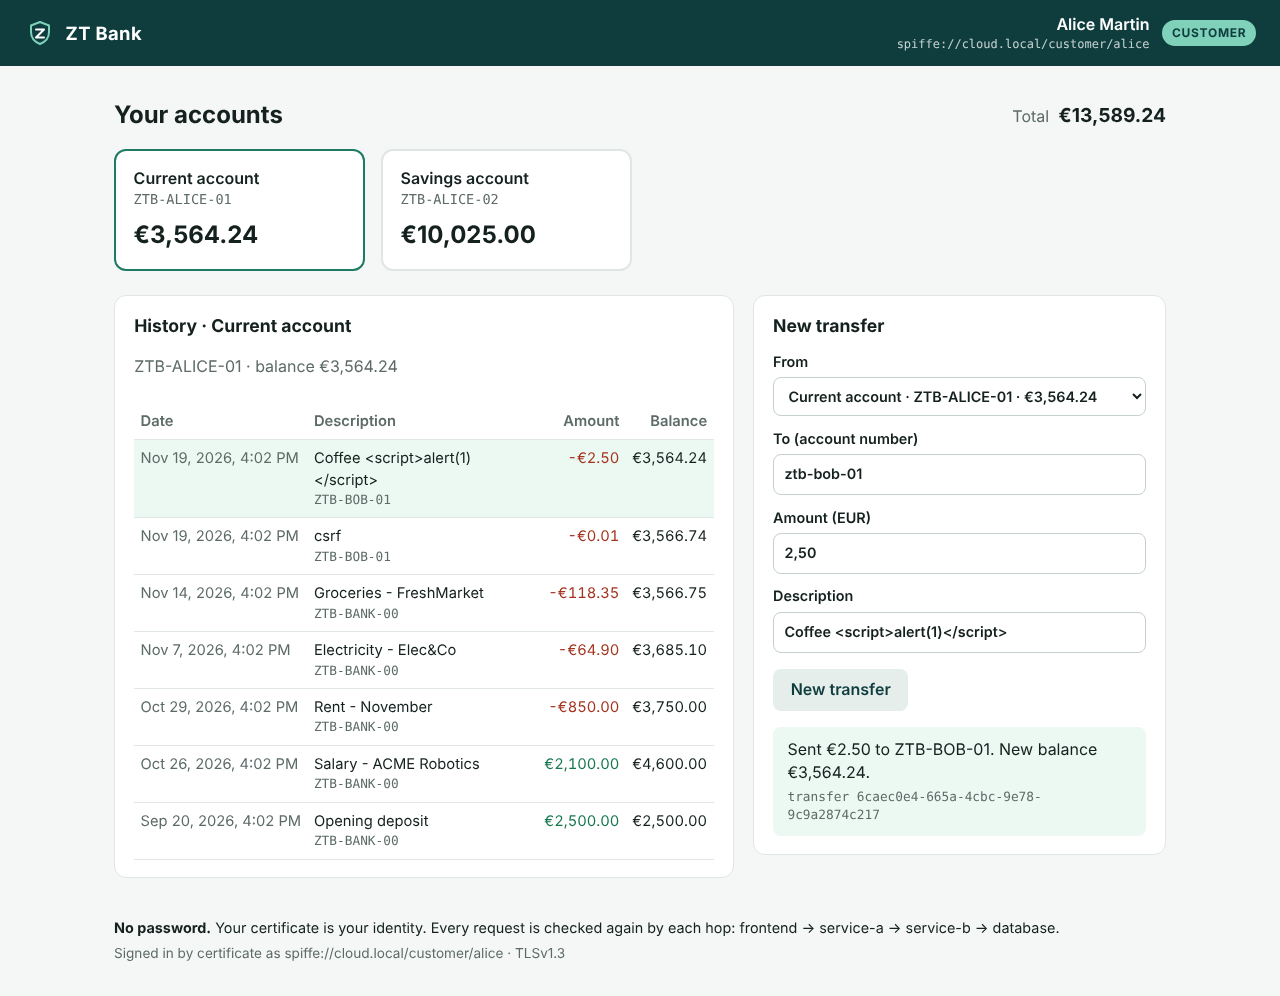
\includegraphics[width=0.62\linewidth]{../screens/customer-alice.png}}{\fbox{capture customer-alice.png}}
\caption{Alice connectée par son seul certificat (données fictives). La description
\cmd{<script>alert(1)</script>} est affichée comme du texte : pas d'injection.}
\end{figure}
\begin{figure}[H]
\centering
\IfFileExists{../screens/staff-dev.png}{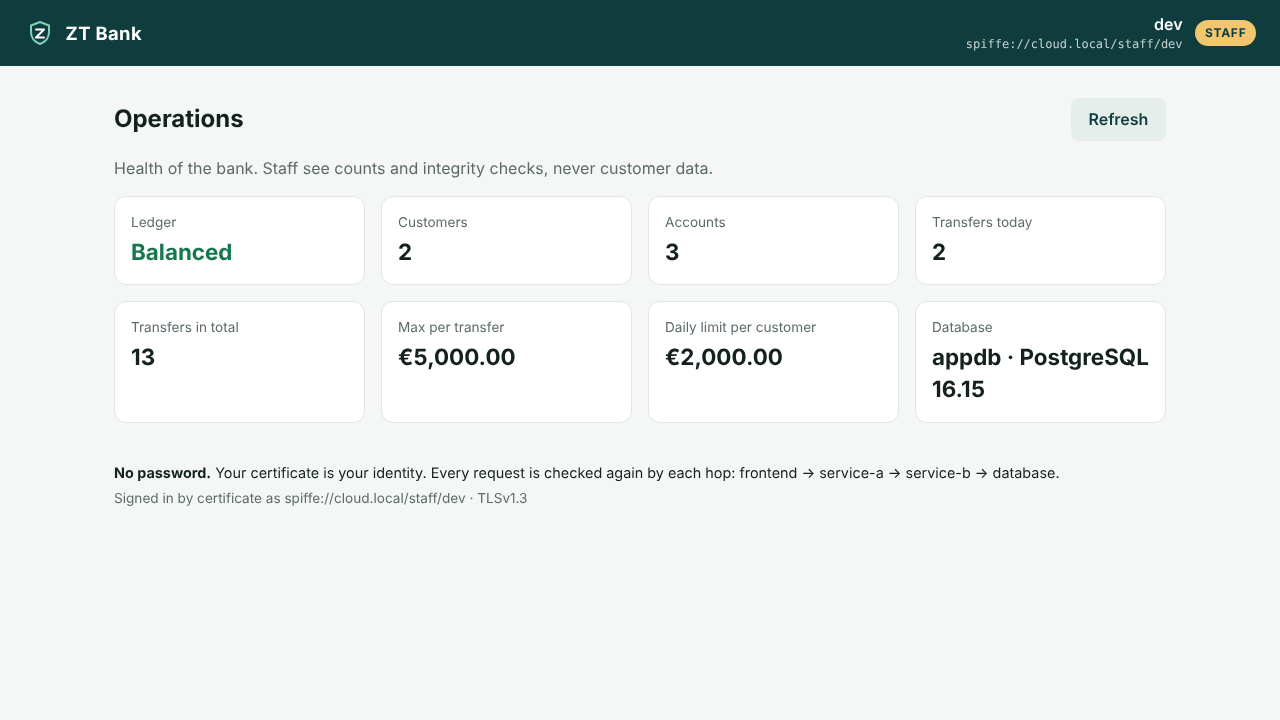
\includegraphics[width=0.48\linewidth]{../screens/staff-dev.png}}{\fbox{capture staff-dev.png}}\hfill
\IfFileExists{../screens/bot-statements.png}{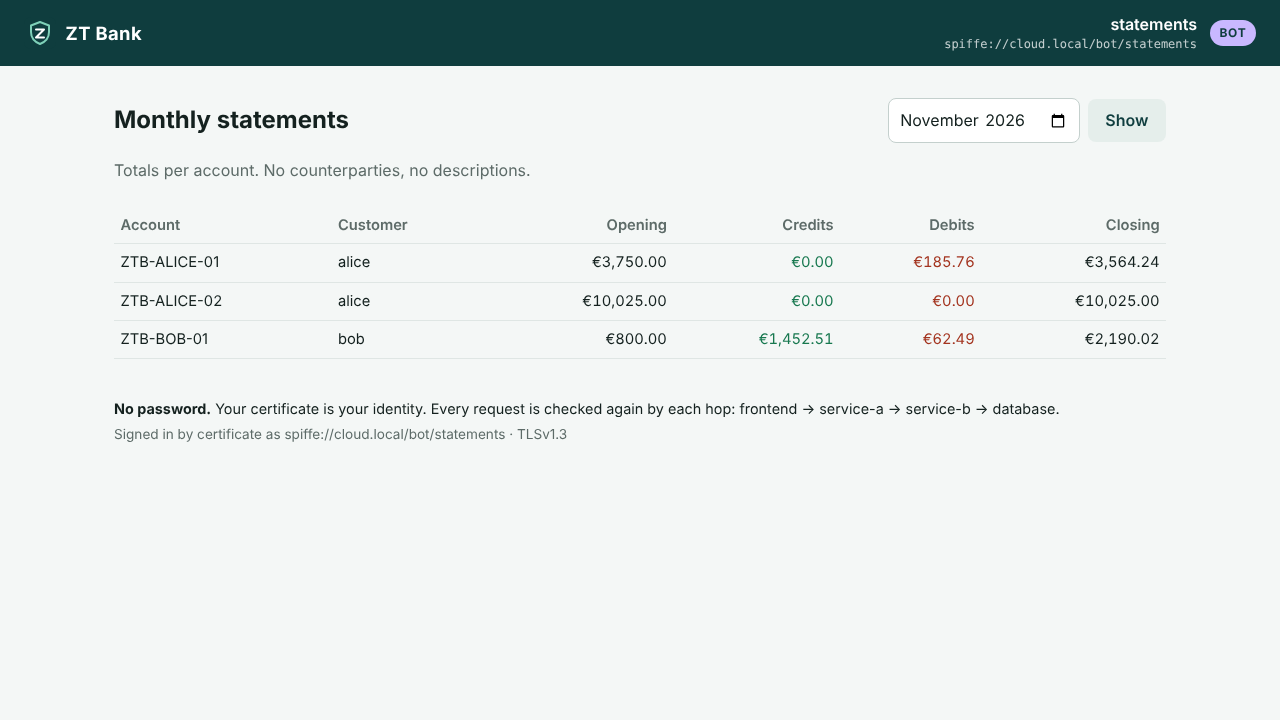
\includegraphics[width=0.48\linewidth]{../screens/bot-statements.png}}{\fbox{capture bot-statements.png}}
\caption{À gauche, Dev (staff) : santé du système, aucune donnée client. À droite, les relevés du robot.}
\end{figure}

% ========================================================== 5. validation ==
\section{Validation}

\subsection{Stratégie de test}
Deux niveaux : plus de 350 tests \textbf{hors ligne} (sans VM : politique, générateur, vrais
programmes lancés localement avec de vrais certificats, banque sur un vrai PostgreSQL, site dans un
vrai navigateur) et des tests \textbf{en direct} sur les VM pour chaque étape. Chaque refus est testé
autant que chaque succès ; les tests de confidentialité contiennent un témoin (un paquet en clair
\emph{doit} être capturé) ; la configuration réelle est comparée à une génération fraîche ; aucun
test n'affiche de secret ; un test vérifie que le dépôt ne contient aucune donnée personnelle.

\subsection{Attaques depuis le cloud host}
\cmd{make attacks} rejoue le catalogue et écrit un rapport. Résultat : \textbf{119 tests réussis sur 119}.
\begin{center}
\begin{tabularx}{\linewidth}{@{}lL l@{}}
\toprule
& \textbf{Attaque} & \textbf{Verdict}\\
\midrule
A1 & Portable volé : copie du certificat d'Alice, révoquée & \defended\\
A2 & Frontend compromis (root sur la VM exposée) & \defended\\
A3 & Mouvement latéral depuis le VPN, usurpation d'adresse & \defended\\
A4 & Identités forgées (autre CA, expirée, aucune, autre identité) & \defended\\
A5 & Scans TCP complets du tunnel et de l'extérieur & \defended\\
A6 & Clé WireGuard volée sans la clé pré-partagée & \defended\\
A7 & Client qui déborde : IDOR, en-têtes forgés, autres rôles & \defended\\
A8 & CSRF depuis une page malveillante & \defended\\
A9 & Notification de paiement forgée ou rejouée & \defended\\
A10 & Inondation de requêtes et de connexions & \defended\\
A11 & Écoute réseau et déclassement (TLS 1.2, clair) & \defended\\
\bottomrule
\end{tabularx}
\end{center}

\subsection{Attaques depuis le poste distant}
Le script \cmd{remote-client/attack.py}, lancé depuis le second ordinateur, lit toutes les adresses
dans la politique et affiche pour chaque sonde « REFUSED (as expected) » ou « BREACH ».
\begin{center}
\begin{tabularx}{\linewidth}{@{}lL l@{}}
\toprule
& \textbf{Sonde} & \textbf{Verdict}\\
\midrule
B1 & Scan des 65\,535 ports du cloud host depuis le Wi-Fi ; seul le port partenaire présente le certificat de la banque & \defended\\
B2 & Site sans certificat, certificats autosignés, TLS 1.2 & \defended\\
B3 & Tous les réseaux de la banque routés dans le tunnel, 13 cibles internes, usurpation d'adresse & \defended\\
B4 & Alice : compte de Bob, en-têtes forgés, routes staff/bot, CSRF ; Dev : données client & \defended\\
B5 & Paiements forgés depuis Internet ; solde inchangé & \defended\\
B6 & Révocation en direct : le certificat d'Alice et Firefox refusés & \defended\\
\bottomrule
\end{tabularx}
\end{center}

\subsection{Audit}
\cmd{make audit} rassemble, en lecture seule, les requêtes par identité, chaque refus avec sa raison,
la CRL appliquée par chaque service, les expirations de certificats, les rejets du pare-feu, l'audit
de la banque, l'équilibre du grand livre et les rapports d'attaques. Résultat final :
\textbf{aucune anomalie}.

\subsection{Ce que les tests ont permis de corriger}
Les tests ne se sont pas contentés de confirmer : ils ont trouvé de vrais défauts pendant la
réalisation, par exemple un verrouillage SSH au premier chargement du pare-feu (corrigé par des
réponses SSH sans état et un retour arrière automatique), une erreur interne 500 au lieu d'un 502
lorsqu'un serveur amont est révoqué, un test qui affichait une clé WireGuard en cas d'échec (clés
régénérées, assertions passées en booléens), et une hypothèse fausse du scanner du poste distant
qui jugeait les ports à leur numéro au lieu de leur certificat.

% ========================================================= démonstration ==
\section{Démonstration}
La démonstration se joue sur les deux machines avec deux scripts Python commentés,
\cmd{tools/demo.py} (cloud host) et \cmd{remote-client/demo.py} (poste distant). Chaque script
affiche ce qu'il fait, lance les vraies commandes, \textbf{anonymise} tout ce qui s'affiche
(utilisateur, nom de machine, dossier personnel, adresse Wi-Fi, adresses MAC) et enregistre une
transcription par scène ; \cmd{tools/render\_captures.py} en fait les captures ci-dessous.
Le scénario complet et l'ordre entre les deux machines sont dans \cmd{docs/24-scenario-demo.md}.

\begin{center}
\begin{tabularx}{\linewidth}{@{}l L l L@{}}
\toprule
\multicolumn{2}{@{}l}{\textbf{Cloud host}} & \multicolumn{2}{l@{}}{\textbf{Poste distant}}\\
\midrule
C1 & le cloud et sa politique & R1 & le tunnel WireGuard\\
C2 & isolation réseau (scan depuis le tunnel) & R2 & Alice dans Firefox, sans mot de passe\\
C3 & les identités décident (IDOR, en-têtes, CSRF) & R3 & Dev : même poste, autres droits\\
C4 & robot et partenaire PayFlow (rejeu refusé) & R4 & identités forgées, débordements (B2, B4)\\
C5 & catalogue d'attaques A1--A11 & R5 & mouvement latéral (B3)\\
C6 & révocation en direct & R6 & scan et faux paiements depuis le Wi-Fi (B1, B5)\\
C7 & nouveau certificat pour Alice & R7 & révocation vue du poste distant (B6)\\
C8 & audit & R8 & nouveau certificat importé dans Firefox\\
\bottomrule
\end{tabularx}
\end{center}

\subsection{L'infrastructure, en direct}
Ces captures montrent le système réel en fonctionnement : les VM dans le gestionnaire de
virtualisation, leur position sur les réseaux lue dans libvirt, les flux actifs lus sur chaque VM,
le tunnel vu du gateway et le trafic chiffré capturé sur un pont (outil \cmd{tools/infra-view.py},
guide : \cmd{docs/25-capturer-l-infrastructure.md}).
\capture[0.85]{infra-virt-manager-vms.png}{Les six VM en fonctionnement (virt-manager).}
\capture[0.85]{infra-virt-manager-reseaux.png}{Les réseaux virtuels : wan en NAT, les autres isolés.}
\capture[0.85]{infra-virt-manager-nic-frontend.png}{Le frontend : une interface sur dmz, une sur app, une sur mgmt.}
\capture{infra-carte-graphique.png}{Carte graphique en direct (navigateur) : VM, réseaux, tunnel, flux actifs animés et paquets rejetés, lus sur le système réel.}
\capture{infra-carte-vivante.png}{Carte vivante : VM, tunnel et flux actifs pendant qu'Alice utilise la banque.}
\capture{infra-vms.png}{Chaque VM et ses réseaux, lus dans libvirt.}
\capture{infra-connexions.png}{Les connexions établies, de bout en bout : tunnel → frontend → service-a → service-b → base.}
\capture{infra-tableau-de-bord.png}{Tableau de bord en direct : carte, connexions, tunnel, rejets du pare-feu.}
\capture[0.85]{infra-wireshark-tls13.png}{Trafic capturé sur le pont app : uniquement du TLS 1.3 chiffré.}

\subsection{Le poste distant : l'utilisateur}
\capture[0.8]{firefox-alice-comptes.png}{R2 — Alice dans Firefox : ses comptes, sans écran de connexion.}
\capture[0.8]{firefox-alice-virement.png}{R2 — Un virement vers Bob ; la description \texttt{<script>} reste du texte.}
\capture[0.8]{firefox-dev-operations.png}{R3 — Dev, depuis le même poste : la santé du système, aucun compte.}
\capture{remote-client-R1.png}{R1 — Le tunnel : une seule route, celle du site.}
\capture{remote-client-R4.png}{R4 — Identités forgées et débordements d'Alice : tout est refusé.}
\capture{remote-client-R5.png}{R5 — Tous les réseaux internes routés dans le tunnel : seul le site répond.}
\capture{remote-client-R6.png}{R6 — Depuis le Wi-Fi : un seul service de la banque publié ; faux paiements refusés.}

\subsection{Le cloud host : l'exploitation}
\capture{cloud-host-C1.png}{C1 — Les six VM et la politique.}
\capture{cloud-host-C2.png}{C2 — Scan depuis le client VPN hostile : seul le port du site répond ; rejets journalisés.}
\capture{cloud-host-C3.png}{C3 — Bob face au compte d'Alice, en-têtes forgés, Dev, CSRF.}
\capture{cloud-host-C4.png}{C4 — Le robot, un paiement PayFlow, une requête rejouée et une requête modifiée.}
\capture{cloud-host-C5.png}{C5 — Le catalogue d'attaques et une attaque rejouée en direct.}

\subsection{Le portable volé}
\capture{cloud-host-C6.png}{C6 — Révocation du certificat d'Alice ; la copie volée est refusée.}
\capture{remote-client-R7.png}{R7 — Le poste distant voit le refus en moins d'une minute.}
\capture[0.8]{firefox-alice-revoquee.png}{R7 — Firefox, rechargé : le certificat révoqué est refusé.}
\capture{cloud-host-C7.png}{C7 — Une nouvelle clé et un nouveau certificat pour Alice.}
\capture{remote-client-R8.png}{R8 — Le nouveau certificat récupéré et importé dans Firefox.}
\capture[0.8]{firefox-alice-nouveau-certificat.png}{R8 — Alice retrouve ses comptes.}
\capture{cloud-host-C8.png}{C8 — L'audit final : aucune anomalie.}

% ============================================================ 6. risques ==
\section{Risques résiduels et perspectives}
\begin{itemize}
  \item \textbf{Frontend compromis} : il parle au nom des clients ; root sur cette VM peut agir comme
        n'importe quel client, dans les limites des routes client et des plafonds. Il n'atteint ni le
        grand livre ni la base, ne détient aucune autre clé. Piste : requêtes signées par la clé du client.
  \item \textbf{Le cloud host} détient toutes les clés et est l'hyperviseur ; le scan du poste distant
        a montré qu'il expose au Wi-Fi ses propres services (SSH, outils de développement), étrangers à
        la banque. Pistes : pare-feu de l'hôte, services liés à 127.0.0.1, chiffrement du disque.
  \item \textbf{La VM ca} : sa compromission permettrait d'émettre des identités. Piste : racine hors ligne, HSM.
  \item \textbf{Latence de révocation} $\leq$ 60~s (immédiate via \cmd{make revoke}).
  \item \textbf{PostgreSQL} ne consulte pas la CRL (son seul client, service-b, est épinglé).
  \item \textbf{Disponibilité} : une VM par rôle, pas de redondance.
  \item \textbf{Post-quantique} : TLS et WireGuard utilisent X25519 / P-256 ; un trafic enregistré
        pourrait être déchiffré plus tard. Perspectives : échange de clés hybride
        X25519MLKEM768 (pris en charge à partir d'OpenSSL~3.5) pour les sauts TLS, et une clé
        pré-partagée post-quantique pour WireGuard (projet Rosenpass). La clé pré-partagée
        actuelle ajoute déjà une couche symétrique au tunnel.
\end{itemize}

% ============================================================ 7. tutoriel ==
\section{Tutoriel : installer et utiliser}
Le guide complet, commande par commande, est dans \cmd{docs/03-reproduire-pas-a-pas.md}.

\subsection{Prérequis}
Cloud host : processeur avec virtualisation activée, 16~Go de RAM, 40~Go libres, Ubuntu 22.04 ou
24.04, Terraform $\geq$ 1.5, ansible-core $\geq$ 2.15, une clé SSH. Poste distant : Linux avec
Firefox, \cmd{wireguard-tools}, \cmd{libnss3-tools}. Les deux sur le même réseau local.

\subsection{Installation}
\begin{lstlisting}
git clone https://github.com/Yassminefeki/PQC-Cloud-Lab.git zerotrust-cloud
cd zerotrust-cloud
cp env.example.yaml env.yaml      # puis éditer entry_point et wan_interface
make test-0                       # vérifications hors ligne
make up                           # tout construire (sudo demandé une fois)
make test                         # toutes les étapes, en direct
\end{lstlisting}

\subsection{Préparer le poste distant}
\begin{lstlisting}
# cloud host : produit build/export/remote-client/ (wg0.conf, alice/, dev/)
make wireguard client-certs
# poste distant, après copie par un canal de confiance :
sudo install -m 600 wg0.conf /etc/wireguard/wg0.conf && sudo wg-quick up wg0
firefox -CreateProfile zt-alice     # importer root_ca.crt et alice.p12 :
# certutil / pk12util (voir docs/19-poste-distant.md)
firefox -P zt-alice --no-remote https://10.20.0.10:8443/
\end{lstlisting}

\subsection{Utiliser}
\begin{center}
\begin{tabularx}{\linewidth}{@{}p{5.2cm}L@{}}
\toprule
\textbf{Action} & \textbf{Commande}\\
\midrule
Se connecter comme Alice & Firefox, profil \cmd{zt-alice}\\
Lancer le robot de relevés & \cmd{make bot-run}\\
Simuler un paiement entrant & \cmd{make pay TO=ZTB-ALICE-01 AMOUNT=10.00}\\
Déclarer un portable volé & \cmd{make revoke ACTOR=alice}, puis \cmd{make client-certs}\\
Rejouer les attaques & \cmd{make attacks} (rapport \cmd{build/reports/attacks.md})\\
Attaquer depuis le poste distant & \cmd{python3 remote-client/attack.py --cloud-host <adresse>}\\
Auditer & \cmd{make audit} (rapport \cmd{build/reports/audit.md})\\
Démonstration commentée & \cmd{make demo}\\
Tout arrêter & \cmd{make destroy}\\
\bottomrule
\end{tabularx}
\end{center}

% ========================================================== conclusion ==
\section{Conclusion}
Le projet montre qu'un modèle zero trust complet tient sur un seul portable : trois verrous
indépendants à chaque saut, des identités de courte durée, le moindre privilège jusque dans la base
de données, une révocation effective en moins d'une minute et une journalisation qui nomme le vrai
responsable de chaque refus. Le choix décisif a été d'écrire la politique une seule fois et d'en
générer à la fois la configuration \emph{et} les tests : la sécurité n'est pas affirmée, elle est
mesurée, et toute dérive est détectée. Les attaques jouées depuis les deux machines ont toutes été
repoussées, et les risques qui restent sont identifiés et documentés.

\appendix
\section{Arborescence du dépôt}
\begin{lstlisting}
policy.yaml            la politique (source unique de vérité)
env.example.yaml       modèle de env.yaml (propre à la machine, non versionné)
Makefile               une cible par étape et par test
tools/                 générateur, robot, partenaire, attaques, audit, démo
terraform/             réseaux et VM libvirt
ansible/               playbooks et rôles (host, ca, nftables, wireguard, pki-client, app, postgres)
tests/unit/            tests hors ligne        tests/<étape>/   tests en direct
tests/attacks/         catalogue A1-A11 et attaques en direct
remote-client/         suite d'attaques B1-B6 pour le poste distant
docs/                  documentation détaillée, modèle de menace, ce rapport
\end{lstlisting}

\end{document}
